\subsubsection{Injektiv}
$\mathbb{R} \mapsto \mathbb{R}^n \Leftrightarrow f(x) = f(y) \Rightarrow x = y$:\\
\bullet \, Jedes Element der Zielmenge höchstens einmal als Funktionswert\\
\bullet \, Alle x von $\mathbb{D}$ können genau ein y von $\mathbb{W}$ durch $f(x)$ erhalten.
$\mathbb{W}$ muss nicht aber kann aber vollständig agbedeckt sein.

\begin{minipage}{0.4\linewidth}
    % Injective Function
    \begin{tikzpicture}[
        scale=0.7,
        set/.style={ellipse, draw, minimum width=2cm, minimum height=3cm},
        element/.style={circle, fill=black, inner sep=1pt}]
    
    % Domain (left set)
    \node[set] (A) at (1.5,0) {$\mathbb{D}$};
    \node[element,label=left:$a$] (a) at (1.5,1) {};
    \node[element,label=left:$b$] (b) at (1.5,0.5) {};
    \node[element,label=left:$c$] (c) at (1.5,-0.5) {};
    
    % Codomain (right set)
    \node[set] (B) at (4,0) {$\mathbb{W}$};
    \node[element,label=right:$1$] (1) at (4,1) {};
    \node[element,label=right:$2$] (2) at (4,0.5) {};
    \node[element,label=right:$3$] (3) at (4,-0.5) {};
    \node[element,label=right:$4$] (4) at (4,-1) {};
    
    % Arrow mappings
    \draw[->,blue] (a) to[bend left] (1);
    \draw[->,red] (b) to (2);
    \draw[->,green!70!black] (c) to[bend right] (3);
    \end{tikzpicture}
\end{minipage}
\hfill
\begin{minipage}{0.49\linewidth}
    % Injective function (e^x)
    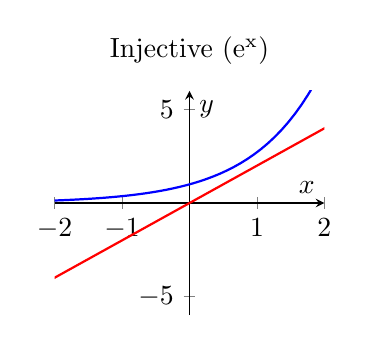
\begin{tikzpicture}
    \begin{axis}[
        scale=0.5,
        axis lines=middle,
        xlabel=\(x\),
        ylabel=\(y\),
        xmin=-2, xmax=2,
        ymin=-6, ymax=6,
        samples=100,
        title={Injective (e\textsuperscript{x})}
    ]
    \addplot[blue, thick] {exp(x)};
    \addplot[red, thick] {2*x};
    \end{axis}
    \end{tikzpicture}
\end{minipage}


\subsubsection{Surjektiv}
$\mathbb{R}^n \mapsto \mathbb{R}$:\\
\bullet \, Jedes Element der Zielmenge mindestens einmal als Funktionswert.\\
\bullet \, $\mathbb{W}$ kann durch $f(x)$ mit x von $\mathbb{D}$ vollständig abgedeckt werden.
\begin{minipage}{0.4\linewidth}
    % Surjective Function
    \begin{tikzpicture}[
        scale=0.7,
        set/.style={ellipse, draw, minimum width=2cm, minimum height=3cm},
        element/.style={circle, fill=black, inner sep=1pt}]
    
    % Domain (left set)
    \node[set] (A) at (1.5,0) {$\mathbb{D}$};
    \node[element,label=left:$a$] (a1) at (1.5,1) {};
    \node[element,label=left:$b$] (b1) at (1.5,0.5) {};
    \node[element,label=left:$c$] (c1) at (1.5,-0.5) {};
    \node[element,label=left:$d$] (d1) at (1.5,-1) {};
    
    % Codomain (right set)
    \node[set] (B) at (4,0) {$\mathbb{W}$};
    \node[element,label=right:$1$] (1) at (4,1) {};
    \node[element,label=right:$2$] (2) at (4,0.5) {};
    \node[element,label=right:$3$] (3) at (4,-0.5) {};
    
    % Arrow mappings
    \draw[->,blue] (a1) to (1);
    \draw[->,red] (b1) to (2);
    \draw[->,green!70!black] (c1) to (3);
    \draw[->] (d1) to[bend right] (3);
    \end{tikzpicture}
\end{minipage}
\hfill
\begin{minipage}{0.4\linewidth}
    % Surjective function (x^3)
    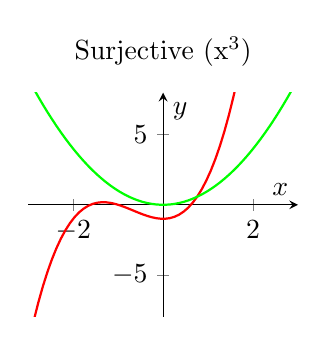
\begin{tikzpicture}
    \begin{axis}[
        scale=0.5,
        axis lines=middle,
        xlabel=\(x\),
        ylabel=\(y\),
        xmin=-3, xmax=3,
        ymin=-8, ymax=8,
        samples=100,
        title={Surjective (x\textsuperscript{3})}
    ]
    \addplot[red, thick] {x^3 + 2*x^2 - 1};
    \addplot[green, thick] {x^2};
    \end{axis}
    \end{tikzpicture}
\end{minipage}



\subsubsection{Bijektiv}
$\mathbb{R} \mapsto \mathbb{R}$\\
\bullet \, Jedes Element der Zielmenge genau einmal als Funktionswert.\\
\bullet \, Bijektive Funktionen haben eine Inverse Funktion.


\begin{minipage}{0.4\linewidth}
    % Bijective Function
    \begin{tikzpicture}[
        scale=0.7,
        set/.style={ellipse, draw, minimum width=2cm, minimum height=3cm},
        element/.style={circle, fill=black, inner sep=1pt}]
    
    % Domain (left set)
    \node[set] (A) at (1.5,0) {$\mathbb{D}$};
    \node[element,label=left:$a$] (a2) at (1.5,1) {};
    \node[element,label=left:$b$] (b2) at (1.5,0.5) {};
    \node[element,label=left:$c$] (c2) at (1.5,-0.5) {};
    
    % Codomain (right set)
    \node[set] (B) at (4,0) {$\mathbb{W}$};
    \node[element,label=right:$1$] (1) at (4,1) {};
    \node[element,label=right:$2$] (2) at (4,0.5) {};
    \node[element,label=right:$3$] (3) at (4,-0.5) {};
    
    % Arrow mappings
    \draw[->,blue] (a2) to[bend left=10] (1);
    \draw[->,red] (b2) to[bend left=0] (2);
    \draw[->,green!70!black] (c2) to[bend right=10] (3);
    \end{tikzpicture}
\end{minipage}
\hfill
\begin{minipage}{0.4\linewidth}
    % Bijective function (linear)
    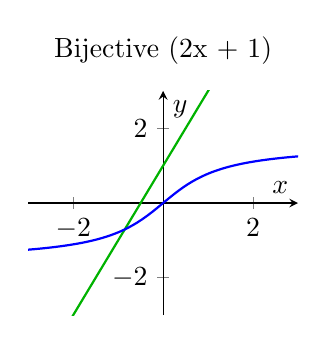
\begin{tikzpicture}
    \begin{axis}[
        scale=0.5,
        axis lines=middle,
        xlabel=\(x\),
        ylabel=\(y\),
        xmin=-3, xmax=3,
        ymin=-3, ymax=3,
        samples=100,
        title={Bijective (2x + 1)}
    ]
    \addplot[green!70!black, thick] {2*x + 1};
    \addplot[blue, thick] {rad(atan(x))};
    \end{axis}
    \end{tikzpicture}
\end{minipage}